% !TEX program = xelatex
% basic document config
\documentclass[a4paper,10pt,xetex]{article}
\usepackage[a4paper,top=45mm,right=20mm,bottom=30mm,left=25mm,head=35mm,foot=20mm]{geometry}

% language
\usepackage[german]{babel}

% variable definitions
\providecommand{\documenttitle}{Anforderungsanalyse}
\providecommand{\documentauthors}{Andreas Saurer \\ Benjamin Schneidinger \\ Josef Erben \\ Raffaele Bof \\ Nicolas Loth}
\providecommand{\documentdate}{28.03.2017}

% special commands
\newcommand*{\fullref}[1]{\hyperref[{#1}]{\nameref*{#1} (\ref*{#1})}}
\newcommand{\specialcell}[2][c]{%
  \begin{tabular}[#1]{@{}l@{}}#2\end{tabular}}

% font
% \usepackage{titling}
\usepackage[sfdefault]{roboto}

% table
\usepackage{array}
\usepackage{multicol}
\usepackage{longtable,tabu,booktabs}

% links
\usepackage{hyperref}
\hypersetup{
            pdftitle={\documenttitle},
            pdfauthor={\documentauthors},
            colorlinks=true,
            linkcolor=[RGB]{74,144,226},
            citecolor=[RGB]{74,144,226},
            urlcolor=[RGB]{74,144,226},
            breaklinks=true}
\urlstyle{same}  % don't use monospace font for urls

% images
\usepackage{float,graphicx,grffile}
\graphicspath{ {images/} }

\makeatletter
\def\maxwidth{\ifdim\Gin@nat@width>\linewidth\linewidth\else\Gin@nat@width\fi}
\def\maxheight{\ifdim\Gin@nat@height>\textheight\textheight\else\Gin@nat@height\fi}
\makeatother
\setkeys{Gin}{width=\maxwidth,height=\maxheight,keepaspectratio}

\makeatletter
\def\fps@figure{H}
\makeatother

% header and footer
\usepackage{lastpage}
\usepackage{fancyhdr}
\pagestyle{fancy}
\fancyhf{}
\fancyhead[L]{
\includegraphics[height=2cm]{travel-buddy_white}}
\fancyfoot[L]{\fontsize{8}{10}\selectfont\ \documenttitle}
\fancyfoot[R]{\fontsize{8}{10}\selectfont\ Seite\ \thepage\ von\ \pageref*{LastPage}}

\renewcommand{\headrulewidth}{0pt}
\renewcommand{\footrulewidth}{0pt}

% style titles
% \usepackage{titlesec}
% \titlespacing*{\section}{0pt}{1em}{0pt}
% \titlespacing*{\subsection}{0pt}{1em}{0pt}
% \titlespacing*{\subsubsection}{0pt}{1em}{0pt}

% configure title page
\title{
  
\includegraphics[width=7cm]{travel-buddy_white}\\[\bigskipamount]
  Anforderungsanalyse\\[\bigskipamount]
}

\author{\documentauthors}
\date{\parbox{\linewidth}{\centering%
  IT15TA ZH \hspace*{3cm} Gruppe 3\endgraf\bigskip
  \documentdate\endgraf
}}


\begin{document}

% title page
\maketitle\newpage

% table of contents
{
\hypersetup{linkcolor=black}
\setcounter{tocdepth}{3}
\tableofcontents
}
\newpage

% version log
\section{Versionenlog}\label{versionenlog}

\tabulinesep=1.2mm

\begin{longtabu} to \textwidth { | l | l | X[l] | l | }
  \hline
  \textbf{Datum} & \textbf{Version} & \textbf{Änderung} & \textbf{Author} \\
  \hline
  \endhead

  0.0.4 & 27.03.2017 & Dokument von Markdown zu Latex für bessere Formatierung konvertiert & A. Saurer\\
  \hline

  0.0.3 & 26.03.2017 & Anwendungsfalldiagramm hinzugefügt & B. Schneidinger\\
  \hline

  0.0.2 & 26.03.2017 & Zusätzliche Spezifikationen definiert & B. Schneidinger\\
  \hline

  0.0.1 & 24.03.2017 & Anwendungsfälle beschrieben und Systemsequenzdiagramm eingebunden & A. Saurer\\
  \hline

  0.0.0 & 21.03.2017 & Dokument erstellt & A. Saurer\\
  \hline
\end{longtabu}
\newpage

% start content
\section{Projektmanagement}\label{projektmanagement}


\subsection{Projektstatus}\label{projektstatus}
Das Projekt befindet sich auf Kurs, der erste Meilenstein wurde erreicht
und der zweite bevorstehende Meilenstein ist fast fertig gestellt. Die
unten gezeigte Grafik zeigt eine grobe Übersicht des Projektes, eine
detaillierte befindet sich im darauf folgenden Abschnitt.

\begin{figure}
  \centering
  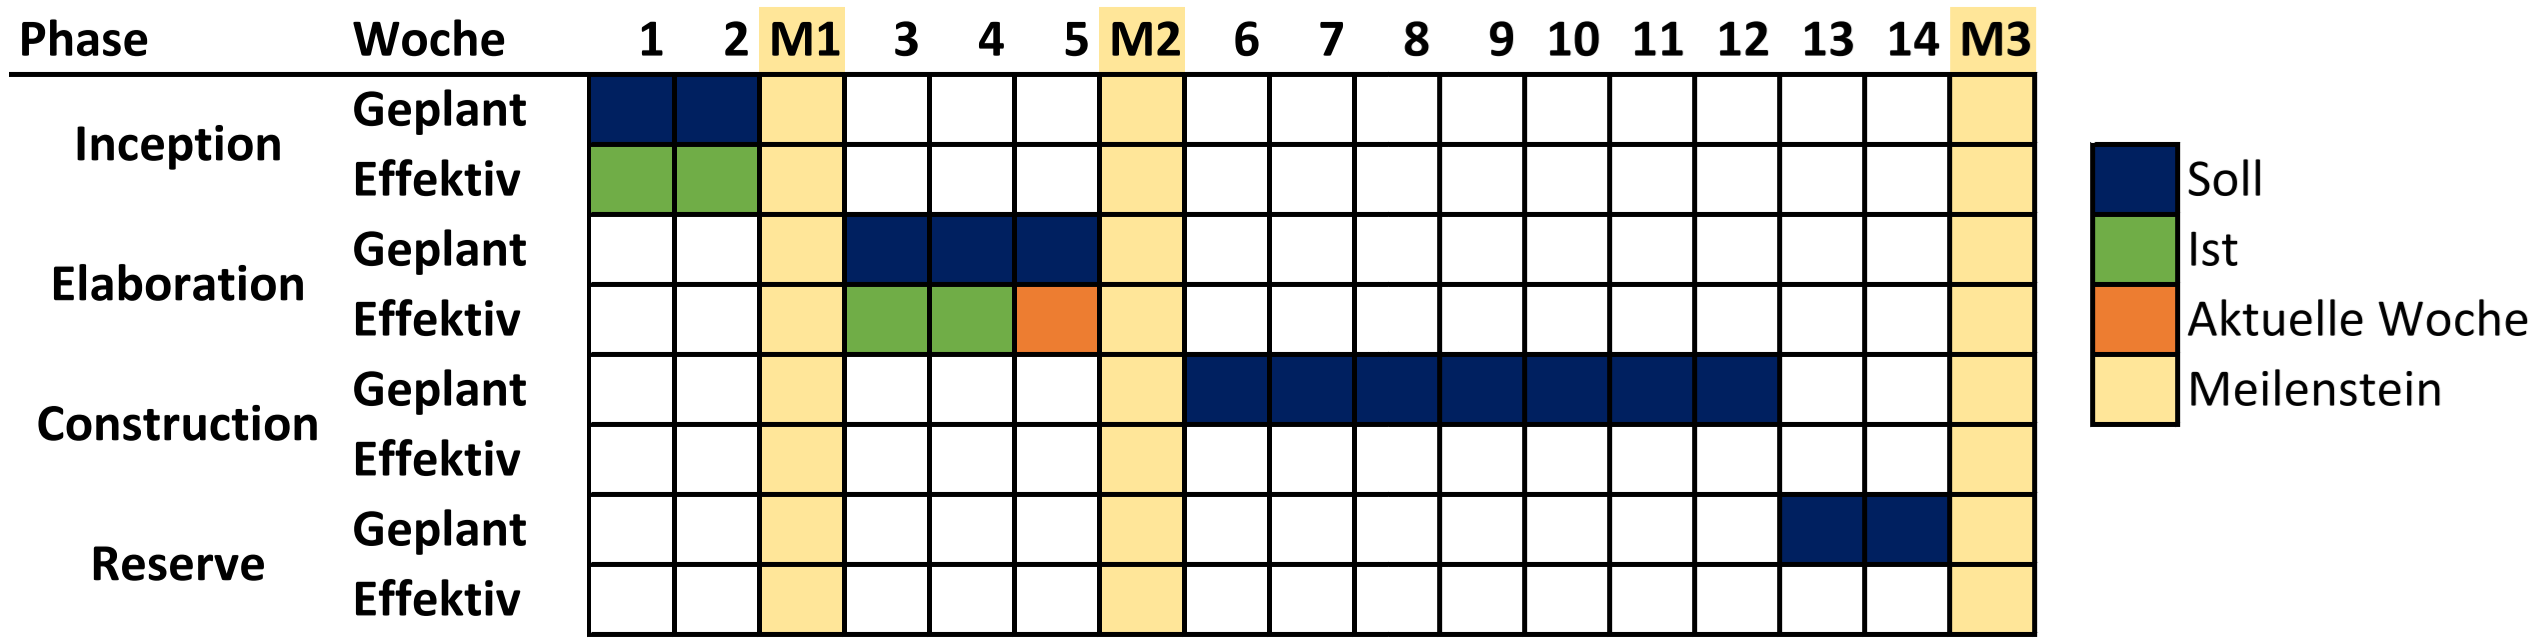
\includegraphics{Grobzeitplan_26.03.2017}
  \caption{Grobzeitplan Stand: 26.03.2017}
\end{figure}


\subsection{Detaillierter Projektplan}\label{detaillierter-projektplan}
\begin{longtabu} to \textwidth { | l | l | X[l] | l | l | }
\hline
\textbf{Phase} & \textbf{Nr.} & \textbf{Arbeitspaket} & \textbf{Soll} & \textbf{Ist} \\\hline
\endhead

\multicolumn{5}{| l |}{ \textbf{Inception} }\\\hline
 & A-01 & Ausgangslage schildern & 5,0 h & \\\hline
 & A-02 & Projektidee beschreiben & 5,0 h & \\\hline
 & A-03 & Kundennutzen analysieren & 5,0 h & \\\hline
 & A-04 & Projektidee beschreiben & 5,0 h & \\\hline
 & A-05 & Konkurenzanalyse & 5,0 h & \\\hline
 & A-06 & Haupablauf aufzeigen & 5,0 h & \\\hline
 & A-07 & Weitere Anforderungen definieren & 5,0 h & \\\hline
 & A-08 & Ressource beschreiben & 5,0 h & \\\hline
 & A-09 & Projektidee beschreiben & 5,0 h & \\\hline
 & A-10 & Risiken beschreiben & 5,0 h & \\\hline
 & A-11 & Grobplanung erstellen & 5,0 h & 3,5 h\\\hline
 & A-12 & Wirtschaftlichkeitsanalyse & 5,0 h & 6,0 h\\\hline
 & A-13 & Projektskizze erstellen (inkl. Präsi) & 5,0 h & \\\hline
Total Phase: & 13 & & 65,0 h & \\\hline
\multicolumn{5}{| l |}{ }\\\hline

\multicolumn{5}{| l |}{ \textbf{Inception} }\\\hline
 & B-01 & Projekmanagement organisieren & 5,0 h & 6,0 h\\\hline
 & B-02 & Anwendungsfall Diagramm zeichnen & 5,0 h & \\\hline
 & B-03 & Domänenmodell erstellen & 5,0 h & \\\hline
 & B-04 & Architektur beschreiben & 5,0 h & \\\hline
 & B-05 & Zusätzliche Spezifikationen beschreiben & 5,0 h & \\\hline
 & B-06 & Syste-Sequenzdiagramm zeichnen & 5,0 h & \\\hline
 & B-07 & Glossar erstellen & 5,0 h & \\\hline
 & B-08 & Use-Case 1 beschreiben & 1,0 h & \\\hline
 & B-09 & Use-Case 2 beschreiben & 0,5 h & \\\hline
 & B-10 & Use-Case 3 beschreiben & 0,5 h & \\\hline
 & B-11 & Use-Case 4 beschreiben & 0,5 h & \\\hline
 & B-12 & Use-Case 5 beschreiben & 0,5 h & \\\hline
 & B-13 & Use-Case 6 beschreiben & 0,5 h & 0,5 h\\\hline
 & B-14 & Analysedokument erstellen (inkl. Präsi) & 6,5 h & \\\hline
Total Phase: & 14 & & 45,0 h & \\\hline
\multicolumn{5}{| l |}{ }\\\hline

\multicolumn{5}{| l |}{ \textbf{Construction} }\\\hline
 & C-01 & Projekmanagement nachtragen & 1,0 h & \\\hline
 & C-02 & UC-1 Liste der verfügbaren Touren & ? h & \\\hline
 & C-03 & UC-1 Starten einer Tour & ? h & \\\hline
 & C-04 & UC-2 Lokalisieren des Benutzers & ? h & \\\hline
 & C-05 & UC-2 Anzeigen des Benutzers auf der Karte & ? h & \\\hline
 & C-06 & UC-3 Foto machen & ? h & \\\hline
 & C-07 & UC-4 Prüfen der Geo koordinaten des Fotos & ? h & \\\hline
 & C-08 & UC-5 Besuchen des nächsten Punktes & ? h & \\\hline
 & C-09 & UC-6 Auslesen der Tourdaten & ? h & \\\hline
 & C-10 & UC-6 Anzeigen der Tourdaten & ? h & \\\hline
 & C-11 & UI gestalten & ? h & \\\hline
 & C-12 & Systemtests durchführen & ? h & \\\hline
 & C-13 & Dokumentation erstellen & ? h & \\\hline
 & C-14 & Benutzeranleitung schreiben & ? h & \\\hline
Total Phase: & 14 & & ? h & \\\hline
\end{longtabu}


\subsection{Risiken}\label{risiken}
\begin{longtabu} to \textwidth { | l | X[l] | l | l | }
\hline
\textbf{Nr.} & \textbf{Risiko} & \textbf{Auswirkung} & \textbf{Wahrscheinlichkeit}\\\hline
\endhead

1 & Schutz der gespeicherten Daten durch unauthorisierte Zugriffe & Schwerwiegend & Hoch\\\hline
2 & Hohe kosten für Anwender Aufgrund der verwendung durch Kartenmaterial & Mittel & Hoch\\\hline
3 & Fehlendes Wissen in der Entwicklung von Mobile Apps & Mittel & Mittel\\\hline
4 & Höhere komplexität durch einbinden von 3 Anbieter Software & Gering & Mittel\\\hline
5 & Keine öffentlichen Karten-API verfügbar & Schwerwiegend & Sehr gering\\\hline
6 & Smartphone GPS koordination ungenau & Gering & Mittel\\\hline
\end{longtabu}


\section{Anwendungsfälle}\label{anwendungsfuxe4lle}
\subsection{UC 1: Tour auswählen und starten(Priorität 1)}\label{uc-1-user-wuxe4hlt-tour-aus-und-startet-die-tour-priorituxe4t-1}
\subsubsection{Primärer Akteur}\label{primuxe4rer-akteur}
Reisende\_r


\subsubsection{Stakeholders und Interessen}\label{stakeholders-und-interessen}
\begin{itemize}
  \item Reisende\_r: Will mit einfachen Schritten eine passende Tour finden und starten.
  \item Premium Tour Anbieter\_in: Will seine Tour prominent plaziert haben um öfters ausgewählt zu werden.
\end{itemize}


\subsubsection{Vorbedingungen}\label{vorbedingungen}
\begin{itemize}
  \item Reisende\_r ist angemeldet.
  \item Touren sind auf Server erfasst.
\end{itemize}


\subsubsection{Erfolgsgarantie}\label{erfolgsgarantie}
Reisende\_r findet eine ansprechende Tour und kann diese starten.


\subsubsection{Standardablauf}\label{standardablauf}
\begin{enumerate}
  \item Reisende\_r öffnet app.
  \item Reisende\_r klickt auf neue Tour starten.
  \item System zeigt Auswahl von Touren an.
  \item Reisende\_r öffnet Filter.
  \item Reisende\_r setzt Filter um gewünschte Tour zu finden.
  \item Reisende\_r klickt auf Tour.
  \item System startet Tour.
  \item Reisende\_r begibt sich zum Startpunkt der Tour.
\end{enumerate}


\subsubsection{Erweiterungen}\label{erweiterungen}
\begin{enumerate}
  \setcounter{enumi}{3}
  \item
    \begin{enumerate}
      \item Auswahl ist abhängig von gerade populären oder von Premium Anbietern beworbenen Touren.
    \end{enumerate}

  \setcounter{enumi}{6}
  \item
    \begin{enumerate}
      \item App zeigt Detailvorschau an.
      \item Benutzer klickt auf Tour starten oder schliessen.
    \end{enumerate}

  \setcounter{enumi}{8}
  \item
    \begin{enumerate}
      \item Die App zeigt dem Benutzer verschiedene Möglichkeiten an, wie er zum Startpunkt kommt.
    \end{enumerate}
\end{enumerate}


\subsubsection{Spezielle Anforderungen}\label{spezielle-anforderungen}
\begin{itemize}
  \item Filtern der Touren muss flüssig reagieren, Resultate werden sofort angezeigt.
\end{itemize}


\subsubsection{Auftrittshäufigkeit}\label{auftrittshuxe4ufigkeit}
Einmal pro Tour.


\subsection{UC 2: Route ablaufen und aktuellen Standort auf Karte betrachten (Priorität 2)}\label{uc-2-user-luxe4uft-route-ab-und-sieht-seine-aktuellen-standort-auf-einer-karte-priorituxe4t-2}
\subsubsection{Erfolgszenario}\label{erfolgszenario}
Tourist\_in befindet sich im Freien zwischen zwei Punkten auf einer
Route, also einer Teilstrecke der Tour. Die App zeigt dem Benutzer seine
aktuelle Position mit einem Marker (z.B. Punkt) an. Die Touristin verlässt
die Route, der Marker zeigt in Echtzeit die Position an, an der sie sich
befindet. Die App berechnet die neue Route mit der aktuellen Postion als
Ausgangslage. Die Reisende kann also zu jederzeit die optimale Route
zwischen ihrer aktuellen Position und dem Ziel nachschauen.


\subsubsection{Erfolgszenario mit Fallback}\label{erfolgszenario-mit-fallback}
Der Tourist befindet sich auf einer Tour durch eine Altstadt. Die App
zeigt dem Benutzer seine aktuelle Position mit einem Marker (z.B. Punkt)
an, der Marker bewegt sich mit dem User mit. Die aktuelle Route zum
nächsten Zwischenziel führt durch ein dicht überdachtes Gebiet. Die App
kann die Position des Users nicht per GPS abfragen, in der Nähe stehen
einige Läden und Restaurants mit WLAN. Die App kann durch eine
Kombination von Standorten von Mobilfunkmasten und WLAN Sendern die
aktuelle Position berechnen. Der Reisende hat kein GPS Signal, aber
sieht sich trotzdem als Punkt auf der Karte in Echtzeit.


\subsection{UC 3: Foto machen am Besichtigungspunkt (Priorität2)}\label{uc-3-user-macht-foto-am-besichtigungspunkt-priorituxe4t-2}
\subsubsection{Erfolgszenario}\label{erfolgszenario-1}
An einem Zielpunkt / Besichtigungspunkt angelangt, wird die Touristin aufgefordert, ein Foto von einem vorgegebenen Objekt zu erstellen. Die
App entscheidet danach ob die Informationen des Fotos mit denjenigen im
System gespeicherten übereinstimmen. Stimmt das Resultat, wird der
nächste Besichtigungspunkt angezeigt.


\subsubsection{Alternativszenario}\label{alternativszenario}
Befindet sich die Touristin nicht am korrekten Ort, wird sie erneut
aufgefordert das vorgegebene Objekt zu fotografieren.


\subsection{UC 4: Bestätigung für Abarbeiten des Punktes erhalten, Route zum nächsten Punkt anschauen (Priorität 2)}\label{uc-4-user-bekommt-bestuxe4tigung-fuxfcr-das-abarbeiten-des-punktes-die-route-zum-nuxe4chsten-punkt-wird-angezeigt.-priorituxe4t-2}
\subsubsection{Erfolgszenario}\label{erfolgszenario-2}
Nach dem korrekten validieren der Position des Touristen, zeigt die App
dem Benutzer den nächsten Besichtigungspunkt mit einem Marker auf einer
Karte an. Von seinem aktuellen Standort wird eine vordefinierte Route
zum nächsten Besichtigungspunkt abgebildet. Der Tourist begibt sich zum
abgebildeten Punkt.


\subsubsection{Alternativszenario}\label{alternativszenario-1}
Der Tourist möchte die Tour unterbrechen und zu einem späteren
Zeitpunkt fortsetzen. Er schliesst die App und kehrt nach unbestimmter
Zeit zurück. Die App zeigt dann den letzten Stand und fragt nach der
Weiterführung oder Abbruch der Tour.


\subsection{UC 5: Nächste Punkte besichtigen bis Tour zu Ende (Priorität 2)}\label{uc-5-user-besucht-nuxe4chste-punkte-bis-tour-zu-ende.-priorituxe4t-2}
UC1 und UC2 werden solange wiederholt, bis die Touristin am Ende der Tour
ist. Hat sie den letzten Punkt erreicht, wird der Touristin der Abschluss
mit einer Nachricht bestätigt und mit UC 6 fortgefahren.


\subsection{UC 6: Statistik der Tour anschauen (Priorität 3)}\label{uc-6-user-sieht-statistik-der-tour.-priorituxe4t-3}
Nach erfolgreichem erreichen des Zielpunktes und dem Abschluss der Tour,
wird dem Tourist eine Übersicht mit Statistiken wie z.B. der total
zurück gelegten Distanz und totale Schritte angezeigt. Durch einen klick
kann der Tourist Fotos, die Statistik und eine Mitteilung auf den
sozialen Medien teilen.


\section{Anwendungsfalldiagramm}\label{anwendungsfalldiagramm}

\begin{figure}
  \centering
  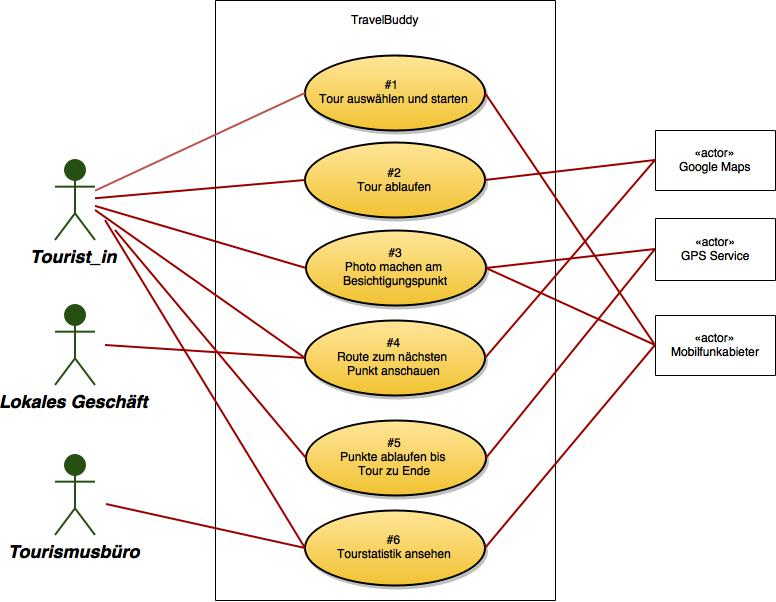
\includegraphics{Anwendungsfalldiagramm}
  \caption{Anwendungsfalldiagramm}
\end{figure}


\section{Domänenmodell}\label{domaenenmodell}
Das folgende Domänenmodell zeigt eine grobe Übersicht der Ausgangslage,
der identifizierten Objekte und Tätigkeiten der Benutzer.

\begin{figure}
  \centering
  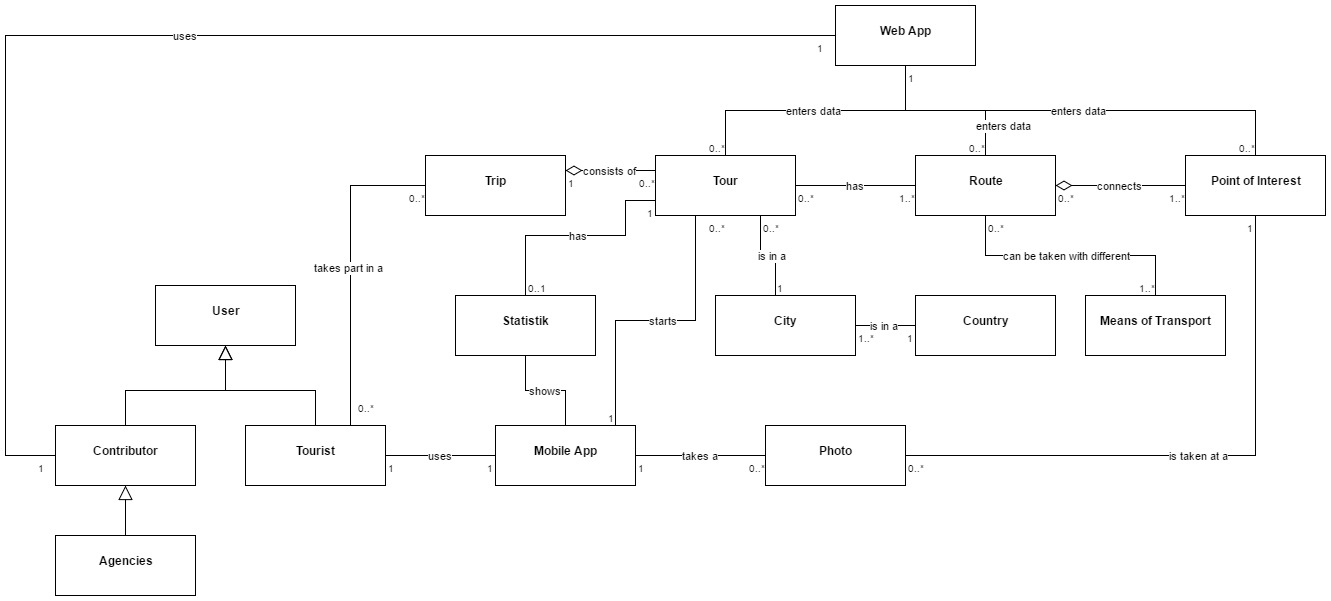
\includegraphics{domain_model1}
  \caption{Domänenmodell}
\end{figure}

\begin{longtabu} to \textwidth { | l | X[l] | }
\hline
\textbf{Objekte} & \textbf{Beschreibung} \\\hline
\endhead

User & Ein Benutzer kann in zwei verschiedenen Rollen auftreten. Als \textbf{Contributor} oder \textbf{Tourist} auftreten.\\\hline
Contributor / Agencies & Ein \textbf{Contributor} erstellt und erfasst Inhalt (d.h.: \textbf{Touren}, \textbf{Routen} und \textbf{Point of Interests}). Ein Subtyp davon sind \textbf{Agencies}, also Reisebüros und Tourismusorganisationen), die als zertifizierte Erfasser agieren.\\\hline
Tourist & Ein \textbf{Tourist} ist der eigentliche Benutzer der,App. Er ist auf Reisen (\textbf{Trip}) und möchte an einem Ort bzw. in einer,Stadt eine \textbf{Tour} unternehmen, um die wichtigsten oder spannendsten \textbf{Point of Interest} kennen zu lernen. Er verwendet dafür die \textbf{Mobile App}.\\\hline
Mobile App & Das ganze Applikations-System ist in zwei Komponenten aufgeteilt. Die \textbf{Mobile App} wird vom \textbf{Touristen} verwendet um sich damit unterstützt entlang einer \textbf{Tour} steuern zu lassen.\\\hline
Web App & Die \textbf{Web App} bietet die funktionale Schnittstelle für \textbf{Contributors}.\\\hline
Trip & Ein \textbf{Tourist} macht eine Reise und hat dort je nach Ort und Stadt mehrere verschiedene \textbf{Touren} zur Auswahl.\\\hline
Tour & Eine \textbf{Tour} ist eine Sammlung von \textbf{Point of Interest}s in einer bestimmten \textbf{Stadt}, die über eine bestimmte \textbf{Route} miteinander verbunden sind.\\\hline
Route & Eine \textbf{Route} stellt eine Verbindung von mehreren \textbf{Point of Interests} dar. Eine Route kann mit verschiedenen \textbf{Verkehrsmitteln} absolviert werden.\\\hline
Point of Interest & \textbf{Point of Interest} sind geographische Punkte, die eine Sehenswürdigkeit oder sonstige spezielle Eigenschaften bieten. Sie werden von einer \textbf{Route} verbunden. Der Tourist muss beim Absolvieren einer Route an jedem \textbf{Point of Interest} vorbeikommen und ein Foto schiessen.\\\hline
Means of Transport & Verschiedene \textbf{Verkehrsmittel} z.B.: ÖV, Auto, Velo, zu Fuss usw\ldots{}\\\hline
Photo & An jedem \textbf{Point of Interest} schiesst der Benutzer mit seiner \textbf{Mobile App} ein \textbf{Foto} des Ortes oder der Sehenswürdigkeit. Die Koordinaten werden abgeglichen und der \textbf{Point of Interest} so als besucht abgehakt.\\\hline
Statistik & Am Ende einer \textbf{Tour}, nachdem alle \textbf{Points of Interest}, besucht wurden, wird dem \textbf{Touristen} eine \textbf{Statistik} über seine absolvierte \textbf{Route}, Anzahl Schritte, Distanz usw\ldots{} angezeigt. Diese ist in der \textbf{Mobile App} verknüpft mit seinen geschossen \textbf{Fotos}.\\\hline
\end{longtabu}


\section{Eine erste Architektur}\label{eine-erste-architektur}
Die Applikation besitzt mehrere Hauptkomponenten:
\begin{itemize}
  \item Mobile Application
  \item Web Service
  \item External Services
  \item Web Application
\end{itemize}
Die Web Application wurde zur besseren Gesamtübersicht in die Darstellung integriert, ist aber nicht Bestandteil der Projekt-Umsetzung und wird daher auch nicht detaillierter beschrieben.

\begin{figure}
\centering
\includegraphics{first_architecture1}
\caption{Erste Architektur}
\end{figure}


\subsection{Mobile Application}\label{mobile-application}
Die Mobile Application wird vom Touristen
verwendet und bietet die Schnittstelle zu den eigentlichen
Hauptfunktionalitäten. Die App wird als 3-tier Applikation aufgebaut. Da
die Daten, auch für eine allfällig zukünftige offline-fähigkeit, sowohl
lokal in der App wie auch über die Data-Services persistiert werden bzw.
zum Beispiel Fotos nur lokal gespeichert werden, teilt sich der
Datenzugriffs-Layer, auf den Persistence Layer und den Data Service
Layer auf. Als vertikaler Layer werden für alle anderen Layer Logging-,
Monitoring- und weitere allgemein verwendete Funktionalitäten zur
Verfügung gestellt.

\begin{longtabu} to \textwidth { | l | X[l] | }
\hline
\textbf{Komponente} & \textbf{Beschreibung} \\\hline
\endhead

Presentation Layer & Implementiert die grafische Schnittstelle zum Benutzer. Weist neben
rudimentärer Eingabe- und Steuerungslogik, neben der Darstellung keine
weiteren Funktionalitäten auf.\\\hline

Business Logic Layer & Hier werden alle App-spezifischen Funktionalitäten implementiert. Dies
beinhaltet zum Beispiel das grafische Aufbereiten der erhaltenen Daten.
Anderseits sind Grundfunktionalitäten wie das Abgleichen der aktuellen
Position mit dem Point of Interest nicht Bestandteil dieses Layer,
sondern serverseitig umgesetzt werden.\\\hline

Persistence Layer & Der Persistence Layer bietet den Datenzugriff auf den lokalen Storage
der App. Damit werden zum Beispiel Fotos gespeichert.\\\hline

Data Service Layer & Dieser Layer bietet den Zugriff auf unseren eigenen Web-Daten-Service,
wie auch auf die Google Maps Services zum Anzeigen der Karte und
Berechnen der Route.\\\hline

Supporting Functionalities & Diese Komponente implementiert alle Funktionalitäten, die den anderen
Komponenten zur Verfügung stehen wie zum Beispiel Logging und sonstige
Monitoring-Funktionalitäten.\\\hline
\end{longtabu}


\subsection{Web Service}\label{web-service}
Der Webservice stellt als Backend-Komponente
sowohl Daten- wie auch funktionale Schnittstelle zur App und zu allen
weiteren Systemen oder externen Systemen dar. Er stellt jederzeit den
aktuellen Referenzdatenstand und alle grundlegenden nicht
zugriffs-system-spezifischen Funktionalitäten an. Dadurch kann eine hohe
Datenqualität und Datenkonsistenz sichergestellt werden. Der Web Service
muss hierfür eine Datenbank-Anbindung zur Persistierung der Daten
aufweisen. Genauso wie die Mobile Application wird der Web Service einen
vertikalen Layer für Logging-, Monitoring- und weitere allgemein
verwendete Funktionalitäten implementieren.

\begin{longtabu} to \textwidth { | l | X[l] | }
\hline
\textbf{Komponente} & \textbf{Beschreibung} \\\hline
\endhead

Data Service Layer & Der Data Service Layer stellt das nach aussen öffentlich verfügbare
Interface zur Verfügung. Er loggt und behandelt ankommende
Requests.\\\hline

Business Logic Layer & Dieser Layer besitzt alle Business-Funktionalitäten, die nicht reine
daten-spezifische Aggregation sind, wie zum Beispiel den Check, ob eine
Koordinate innerhalb eines Points of Interests ist.\\\hline

Persistence Layer & Implementiert sowohl den eigentlichen Datenzugriff, wie auch die
OR-Mapping Logik. Der Layer ist für einen konsistenten, Schreib- und
Lesezugriff auch bei mehreren gleichzeitigen abgearbeiteten Requests
verantwortlich.\\\hline

Supporting Functionalities & Diese Komponente implementiert alle Funktionalitäten, die den anderen
Komponenten zur Verfügung stehen wie zum Beispiel Logging und sonstige
Monitoring-Funktionalitäten.\\\hline
\end{longtabu}


\subsection{External Services}\label{external-services}
Wo bereits Funktionen oder grafische
Komponenten bestehen, werden diese über externe Services bezogen und
eingebunden. Hierbei werden wir in einem ersten Schritt auf öffentlich
zur Verfügung stehende Services zurückgreifen. Als grundlegenden Service
werden die Google Maps Funktionalitäten eingebunden.

Google Maps Services: Die Funktionalitäten zur Anzeige der Karte, den
verschiedenen Point of Interests und zur Berechnung der Route werden
nicht selber implementiert. Hierfür binden wir als externen Service die
Google Maps Services ein. Die Route und die Point of Interests, die vom
eigenen Web-Service geladen werden, werden als Overlay über die
Kartenfunktionalität von Google implementiert.


\subsection{Tech Stack}\label{tech-stack}
Die nachfolgende Tabelle zeigt die eingesetzten Technologien für die
einzelnen System-Komponenten. Innerhalb dieses Projekt-Scopes wird die
Mobile App als native Android App umgesetzt.

\begin{longtabu} to \textwidth { | l | X[l] | }
\hline
\textbf{Komponente} & \textbf{Beschreibung} \\\hline
\endhead

Native Android App & \specialcell{JAVA 8\\Android SDK / Android Studio 2.3}\\\hline
Web Service & \specialcell{.NET Framework 4.5\\C\# 5.0\\ASP.NET Web-API 2.2 (5.2.3)\\Entity Framework 6.0\\Ninject Dependency Injection Framework 3.2}\\\hline
Web Application & \specialcell{.NET Framework 4.5\\C\# 5.0\\ASP.NET MVC 5.2.3 (Razor Engine)\\HTML 5.0\\Angular JS 2.2.4 or React JS 15.4.2\\JQuery 3.2.1}\\\hline
\end{longtabu}


\section{ZusätzlicheSpezifikationen}\label{zusuxe4tzliche-spezifikationen}
\subsection{Einführung}\label{einfuxfchrung}
Hier werden hauptsächlich alle nicht funktionalen Anforderungen
definiert. Die funktionalen Anforderungen sind zum grössten Teil in den
Anwendungsfällen erfasst. An diesem Dokument finden sich nur weitere
funktionale Anforderungen, welche nicht in Zusammenhang mit einem
Anwendungsfall stehen.


\subsection{Funktionalität}\label{funktionalituxe4t}
\subsubsection{Logging / Fehlerbehandlung}\label{logging-fehlerbehandlung}
Benutzer- und Systemaktivitäten sollen lokal auf dem Gerät gespeichert
werden. Im Fehlerfall können diese Informationen an den Server geschickt
und für die Fehleranalyse verwendet werden. Fehlerinformationen sollen
automatisch an den Server geschickt werden.


\subsubsection{Kartenmaterial}\label{kartenmaterial}
Für die Wegweisung soll die Kartenfunktionalität von Google verwendet
werden. Google Maps unterstützt das offline Speichern von bestimmten
Kartenabschnitten, was für Travelbuddy benötigt wird.


\subsubsection{Sicherheit}\label{sicherheit}
Um Touren durchführen zu können, muss sich die Kundin authentifizieren.
Dazu kann der Kunde ein Konto anlegen, oder sich mit seinem Facebook-
oder Google-Konto anmelden.


\subsection{Verwendbarkeit}\label{verwendbarkeit}
\subsubsection{Hardware Limitierung}\label{hardware-limitierung}
Die Applikation soll als Touchscreen-App für Android Geräte entwickelt
werden.


\subsubsection{Lokalisierung}\label{lokalisierung}
Verschiedene Sprachen müssen unterstützt werden können. Reisende wählen
ihre gewünschte Sprache in der App aus. Danach wird das GUI in der
vorgegebenen Sprache angezeigt. Die Touren werden ebenfalls in der
gewünschten Sprache angezeigt, sofern es eine Übersetzung gibt.


\subsubsection{Offline Unterstützung}\label{offline-unterstuxfctzung}
Die Tourensuche funktioniert nur, wenn der Kunde Internetzugang hat.
Einzelne Touren können danach lokal auf dem Gerät des Kunden gespeichert
werden, so dass Reisende eine Tour auch ohne Internetzugang durchführen
können.


\subsubsection{Graphische Oberfläche}\label{graphische-oberfluxe4che}
\begin{itemize}
  \item Konzipiert für Smartphones und Tablets.
  \item Bedienung durch Touchscreen.
\end{itemize}


\subsection{Umsetzungsbedingungen}\label{umsetzungsbedingungen}
Als Entwicklungsprozess wird der Unified Process verwendet. Dies ist ein
populärer, iterativer Software-Entwicklungsprozess um objektorientierte
Systeme zu bauen.\cite{UP}


\subsubsection{Backend}\label{backend}
Für die Umsetzung des Backends sollen folgende Microsoft Technologien
verwendet werden:

\begin{itemize}
  \item Microsoft ASP.NET
  \item Microsoft SQL Server
  \item Microsoft Visual Studio 2015 Enterprise
  \item .NET Framework 4.6
\end{itemize}

Das Backend stellt eine REST API bereit. Das Backend muss in der Lage
sein, Anfragen so schnell beantworten zu können, dass die Anforderungen
an das Reaktionsverhalten der App erfüllt werden können.

\begin{longtabu} to \textwidth { | X[l] | l | }
\hline
\textbf{Benutzer Aktion} & \textbf{Max. Reaktionszeit {[}ms{]}}\\\hline
\endhead

Anmelden & 80\\\hline
Suchen nach Touren & 150\\\hline
Starten von Touren & 400\\\hline
Offline Speichern von Touren & Bandbreiten Abhängig. Daten \textless{} 10 MB\\\hline
Hochladen von Photos und Routenanzeige zum nächsten Standort & 5000 (Photo komprimieren)\\\hline
\end{longtabu}


\subsubsection{App}\label{app}
Es wird eine native Android Applikation entwickelt. Für die Entwicklung
wird verwendet:

\begin{itemize}
  \item Android Studio 2.3
  \item JetBrains IntelliJ
\end{itemize}


\subsection{Zuverlässigkeit}\label{zuverluxe4ssigkeit}
Bei einem Absturtz der App, muss die Reisende nach einem Neustart die
aktuelle Tour weiterführen können. Die App kennt den aktuellen Standort
und rekonstruiert gegebenenfalls die Route zum nächsten Ziel
vollautomatisch.


\section{Systemsequenzdiagram}\label{systemsequenzdiagram}

\begin{figure}
\centering
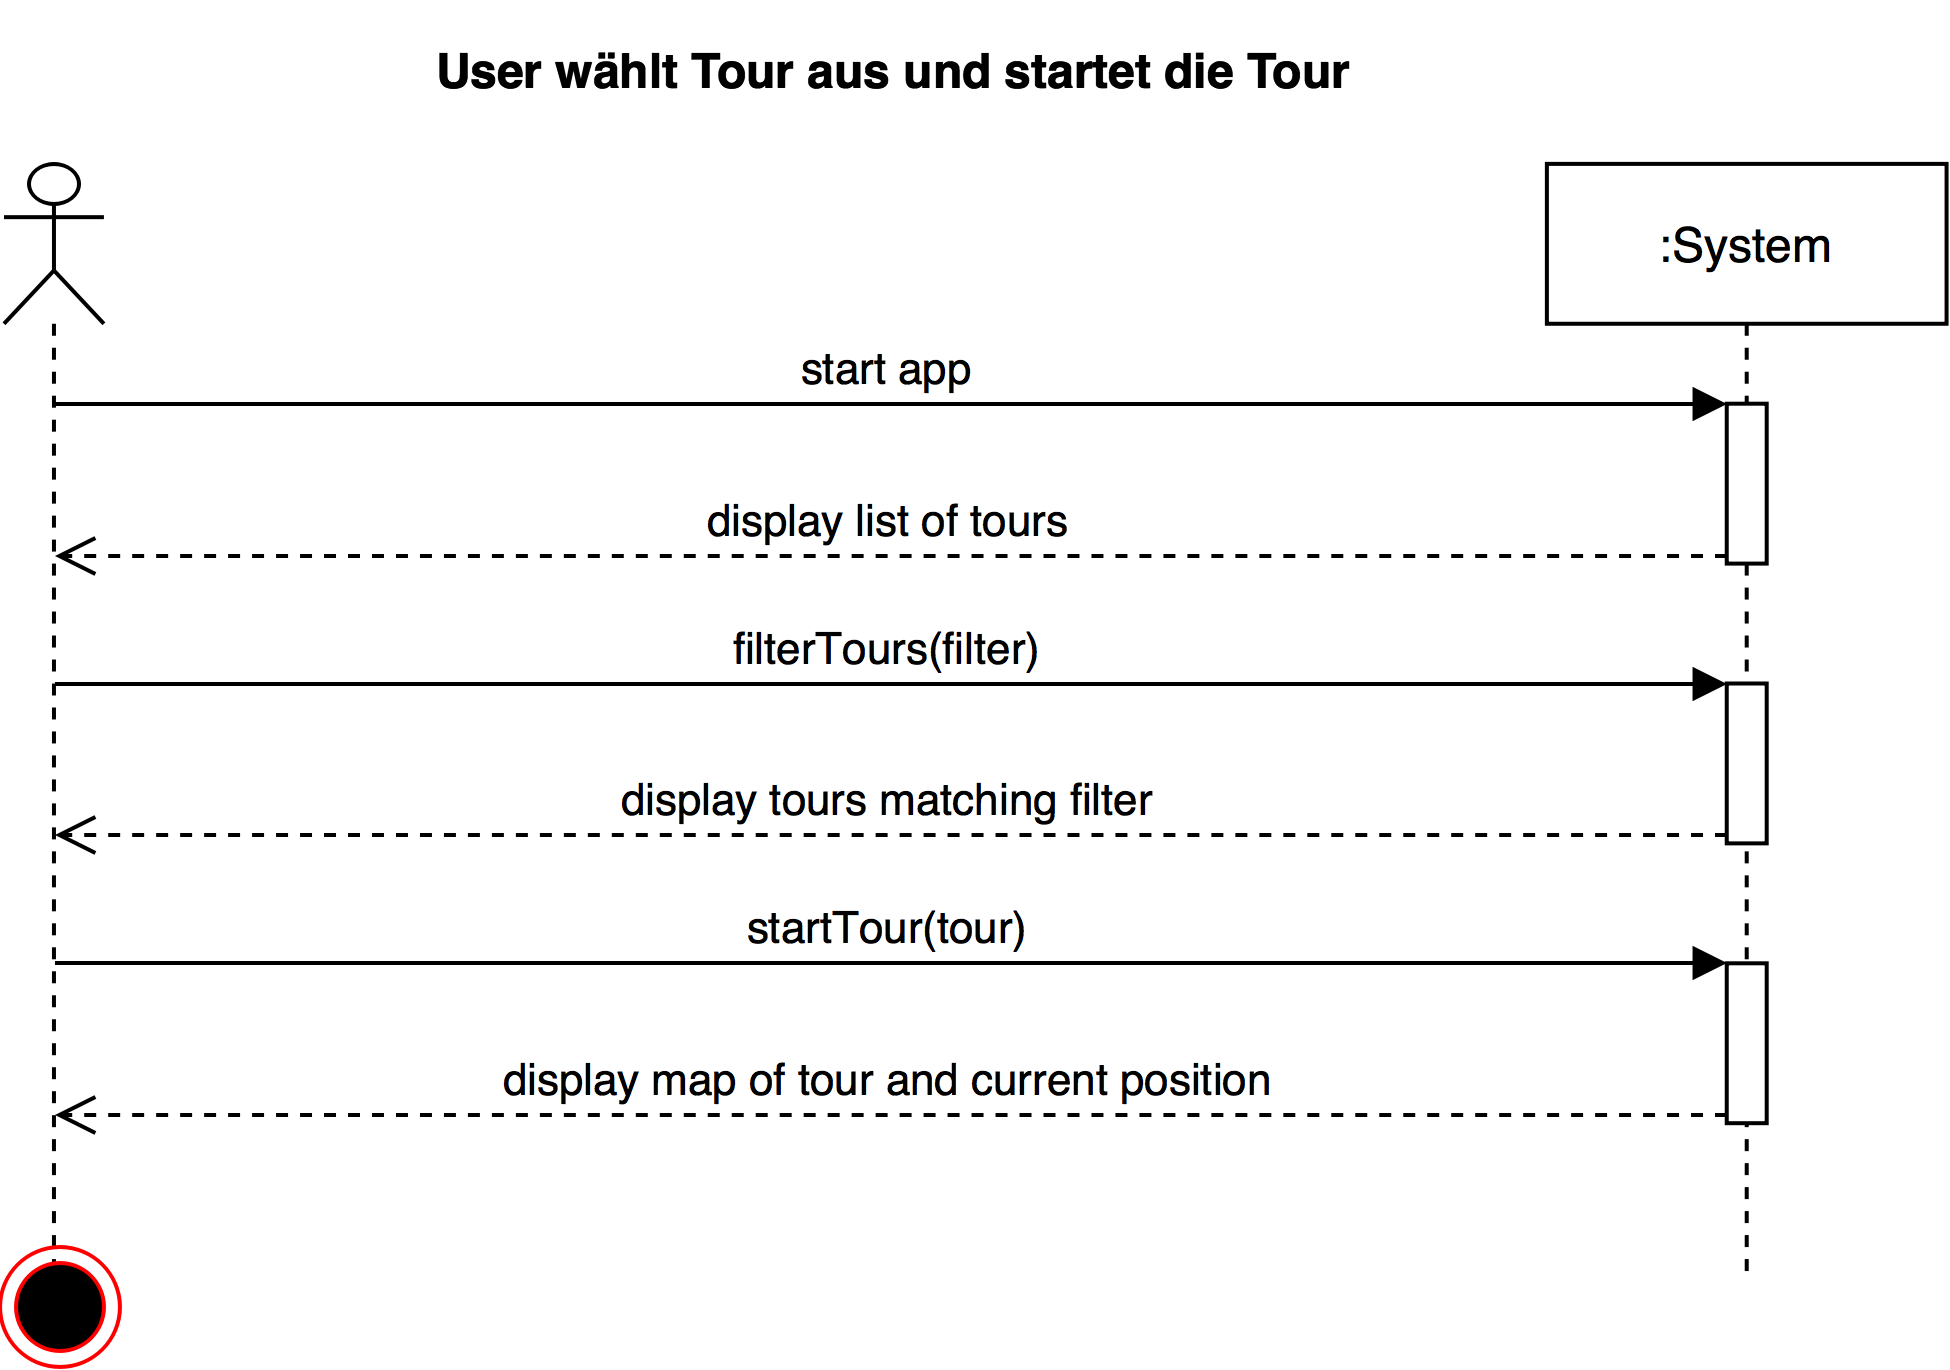
\includegraphics{UC1_SystemSequenzDiagram}
\caption{System Sequenz Diagramm}
\end{figure}


\section{Glossar}\label{glossar}
\begin{longtabu} to \textwidth { | l | X[l] | }
\hline
\textbf{Begriff} & \textbf{Erklärung}\\\hline
\endhead

Agency/Agencies & engl. Agenturen\\\hline
API & Application Programming Interface, eine Schnittstelle zwischen zwei Programmen\\\hline
App & Abkz. Applikation, Synonym für Programm\\\hline
Backend & Serverseitiges Programm das vom Benutzer nur über ein Frontend angesteuert werden kann\\\hline
Business Logic & engl. Geschäftslogik, logischer Ablauf des Programmes\\\hline
Construction-phase & Phase in der das Projekt umgesetzt wird\\\hline
Contributor & engl. Beitragender, jemand der Inhalt für die Applikation erstellt\\\hline
Elaboration-phase & Phase in der das Projekt genauer ausgearbeitet wird\\\hline
External Services & engl. Externe Dienste, Dienste die nicht vom Programm selber ausgeführt werden\\\hline
Fallback & Ausweichlösung/Alternativlösung\\\hline
Frontend & Benutzerseitiges Programm das vom Benutzer direkt gesteuert werden kann\\\hline
GPS & Globa Positioning System, globales Satelliten Navigationsnetz\\\hline
Inception-phase & Gründungsphase, beginn des Projektes\\\hline
Logging & Aufzeichnen von Abläufen im Programm\\\hline
Marker & Symbol das einen Punkt auf der Karte markiert\\\hline
Means of Transport & engl. Verkehrsmittel\\\hline
Meilenstein & Bedeutender Schritt in der Entwicklung\\\hline
Mobile App & Programm dass nur auf einem Mobilgerät ausgeführt werden kann\\\hline
Native & Funktionen die von einem Gerät ohne weitere Software ausgeführt werden kann\\\hline
ÖV & abkz. Öffentlicher Verkehr\\\hline
Point of Interest, PoI & engl. Ort von besonderem Interesse, bspw. Wahrzeichen\\\hline
Ressource & Mittel das zur Entwicklung genutzt werden kann\\\hline
Smartphone & Mobilgerät mit erweiterten Funktionen\\\hline
Stakeholders & engl. Interessenten\\\hline
Tech Stack & Eingesetzte Technologien\\\hline
Trip & engl. Reise\\\hline
Use-Case & engl. Anwendungsfall, Szenarien in der ein Benutzer versucht ein bestimmtes Ziel zu erreichen\\\hline
User & engl. Benutzer\\\hline
Web App & Nur über den Webbrowser benutzbares Programm\\\hline
WLAN & Wireless local area netweork, Kabellose netzwerkverbindung\\\hline
\end{longtabu}


\section{Literatur}\label{literatur}
\begingroup
\renewcommand{\section}[2]{}%
  \begin{thebibliography}{9}
    \bibitem{UP} C. Larman, Applying UML and patterns. 4. Auflage, Upper Saddle River: Pearson Education, Inc., 2005, S. 18.
  \end{thebibliography}
\endgroup

\end{document}
